\documentclass[aspectratio=169,10pt]{beamer}

\usepackage[T1]{fontenc}
\usepackage[utf8]{inputenc}
\usepackage[indonesian]{babel}
\usepackage{amsmath}
\usepackage{amssymb}
\usepackage{tikz}
\usepackage{ragged2e}
\usepackage{array}
\usepackage{graphicx}
\usepackage{hyperref}
\usepackage{booktabs}

\usetikzlibrary{arrows.meta,calc,fit,positioning,shapes.geometric,backgrounds}

\graphicspath{{out/}}

\definecolor{Ink}{HTML}{13293D}
\definecolor{Sky}{HTML}{3E7B9C}
\definecolor{Mist}{HTML}{EAF1F6}
\definecolor{Leaf}{HTML}{DDF0D8}
\definecolor{Sand}{HTML}{FFF2CC}
\definecolor{Rose}{HTML}{F8D7DA}
\definecolor{Slate}{HTML}{5C6770}
\definecolor{SoftBlue}{HTML}{D9E8F5}

\setbeamertemplate{navigation symbols}{}
\setbeamertemplate{footline}[frame number]
\setbeamertemplate{blocks}[rounded][shadow=false]
\setbeamertemplate{itemize item}{\color{Sky}$\blacktriangleright$}
\setbeamertemplate{itemize subitem}{\color{Sky}$\bullet$}
\setbeamertemplate{enumerate item}{\color{Sky}\bfseries\insertenumlabel.}

\setbeamercolor{background canvas}{bg=white}
\setbeamercolor{normal text}{fg=Ink,bg=white}
\setbeamercolor{frametitle}{fg=Ink,bg=white}
\setbeamercolor{framesubtitle}{fg=Slate}
\setbeamercolor{title}{fg=Ink}
\setbeamercolor{block title}{fg=white,bg=Ink}
\setbeamercolor{block body}{fg=Ink,bg=Mist}
\setbeamercolor{footline}{fg=Ink,bg=white}

\setbeamerfont{title}{size=\Large,series=\bfseries}
\setbeamerfont{frametitle}{size=\Large,series=\bfseries}
\setbeamerfont{framesubtitle}{size=\small,shape=\itshape}
\setbeamerfont{block title}{series=\bfseries}

\newcommand{\pill}[2]{%
  \tikz[baseline=(n.base)]\node[rounded corners=8pt, fill=#1, text=Ink, inner xsep=7pt, inner ysep=3pt] (n) {\scriptsize #2};%
}

\newcommand{\sectiontitle}[1]{%
  {\large\bfseries #1}%
}

\begin{document}

% ─────────────────────────────────────────────
%  SLIDE 1 · Judul
% ─────────────────────────────────────────────
\begin{frame}[plain]
  \begin{tikzpicture}[remember picture,overlay]
    \fill[Ink!8]  ([xshift=4.3cm, yshift=-4.8cm]current page.north west) circle (1.2cm);
    \fill[Ink!6]  ([xshift=9.8cm, yshift=-6.4cm]current page.north west) circle (2.1cm);
    \fill[Sky!20] ([xshift=14.5cm,yshift=-2.0cm]current page.north west) circle (1.8cm);
    \fill[Sky!10] ([xshift=1.0cm, yshift=-7.5cm]current page.north west) circle (1.0cm);
  \end{tikzpicture}

  \vfill
  \begin{center}
    \begin{minipage}{0.85\textwidth}
      \centering
      {\color{Sky}\rule{4cm}{2pt}}
      \vspace{0.30cm}
      
      {\usebeamerfont{title}
        Penerapan \textit{Memetic Particle Swarm Optimization} untuk \textit{Traveling Salesperson Problem}
      \par}
      \vspace{0.15cm}
      {\color{Slate}\small Studi Kasus Optimasi Rute Kabupaten/Kota di Jawa Barat}

      \vspace{0.40cm}
      {\color{Sky}\rule{4cm}{1pt}}
      \vspace{0.30cm}
      
      \begin{tabular}{@{}ll@{\hspace{1.4cm}}ll@{}}
        {\color{Ink}\footnotesize Naufal Akmal Rizqulloh} & {\color{Slate}\footnotesize G6401231065} &
        {\color{Ink}\footnotesize Insan Anshary Rasul}    & {\color{Slate}\footnotesize G6401231132} \\[4pt]
        {\color{Ink}\footnotesize Adhiya Radhin Fasya}    & {\color{Slate}\footnotesize G6401231068} &
        {\color{Ink}\footnotesize Daffa Naufal Mumtaz}    & {\color{Slate}\footnotesize G6401231168} \\[4pt]
        {\color{Ink}\footnotesize Faiz Naufal Huda}       & {\color{Slate}\footnotesize G6401231124} & & \\
      \end{tabular}

      \vspace{0.35cm}
      {\color{Slate}\small
        Departemen Ilmu Komputer $\cdot$ IPB University $\cdot$ KOM1326
      }
    \end{minipage}
  \end{center}
  \vfill
\end{frame}

% ─────────────────────────────────────────────
%  SLIDE 2 · Latar Belakang
% ─────────────────────────────────────────────
\begin{frame}{Latar Belakang}
  \framesubtitle{Optimasi Rute dalam Permasalahan Nyata}
  \begin{itemize}
    \item Optimasi rute berperan penting pada distribusi barang, logistik, transportasi, dan layanan publik.
    \item \textbf{Tujuan utama:} Meminimalkan jarak tempuh, waktu perjalanan, dan biaya operasional.
    \item Semakin banyak lokasi yang harus dikunjungi, semakin sulit menentukan urutan perjalanan terbaik.
    \item Penelitian ini menggunakan 27 kabupaten/kota di Jawa Barat sebagai representasi permasalahan nyata.
  \end{itemize}
  \vspace{0.5cm}
  \begin{block}{Pesan Utama}
    Menentukan urutan kunjungan yang optimal merupakan persoalan optimasi yang kompleks.
  \end{block}
\end{frame}

% ─────────────────────────────────────────────
%  SLIDE 3 · TSP
% ─────────────────────────────────────────────
\begin{frame}{Formulasi Masalah: \textit{Traveling Salesperson Problem}}
  \begin{columns}[T]
    \column{0.55\textwidth}
    Diberikan sekumpulan lokasi $V=\{v_1,v_2,\dots,v_n\}$.
    
    Tujuan TSP adalah menemukan rute yang:
    \begin{itemize}
      \item Mengunjungi setiap kota tepat satu kali.
      \item Kembali ke kota awal.
      \item Memiliki total jarak minimum.
    \end{itemize}
    
    \vspace{0.2cm}
    \textbf{Fungsi Objektif:}
    \[
      \min \sum_{i=1}^{n-1} d(\pi_i,\pi_{i+1})+d(\pi_n,\pi_1)
    \]

    \column{0.4\textwidth}
    \begin{block}{Kasus Penelitian}
      \begin{itemize}
        \item 27 titik lokasi
        \item Ruang pencarian $\approx 27!$ ($10^{28}$) kemungkinan.
        \item Masalah \textbf{NP-Hard}.
      \end{itemize}
    \end{block}
    \vspace{0.2cm}
    \footnotesize\color{Slate}
    Enumerasi seluruh kemungkinan rute (\textit{brute-force}) tidak praktis sehingga mutlak diperlukan algoritma optimasi.
  \end{columns}
\end{frame}

% ─────────────────────────────────────────────
%  SLIDE 4 · Dataset & Matriks Jarak
% ─────────────────────────────────────────────
\begin{frame}{Dataset \& Perhitungan Jarak (Haversine)}
  \begin{columns}[T]
    \column{0.45\textwidth}
    \textbf{Data 27 Kabupaten/Kota Jawa Barat}
    \begin{itemize}
      \item Dataset mencakup Nama wilayah, Latitude, dan Longitude.
    \end{itemize}
    
    \vspace{0.4cm}
    \textbf{Kalkulasi Jarak (Haversine)}
    \begin{itemize}
      \item Digunakan karena memperhitungkan kelengkungan permukaan bumi.
      \item Jauh lebih akurat dibandingkan jarak \textit{Euclidean} untuk koordinat geografis nyata.
    \end{itemize}
    
    \column{0.5\textwidth}
    \centering
    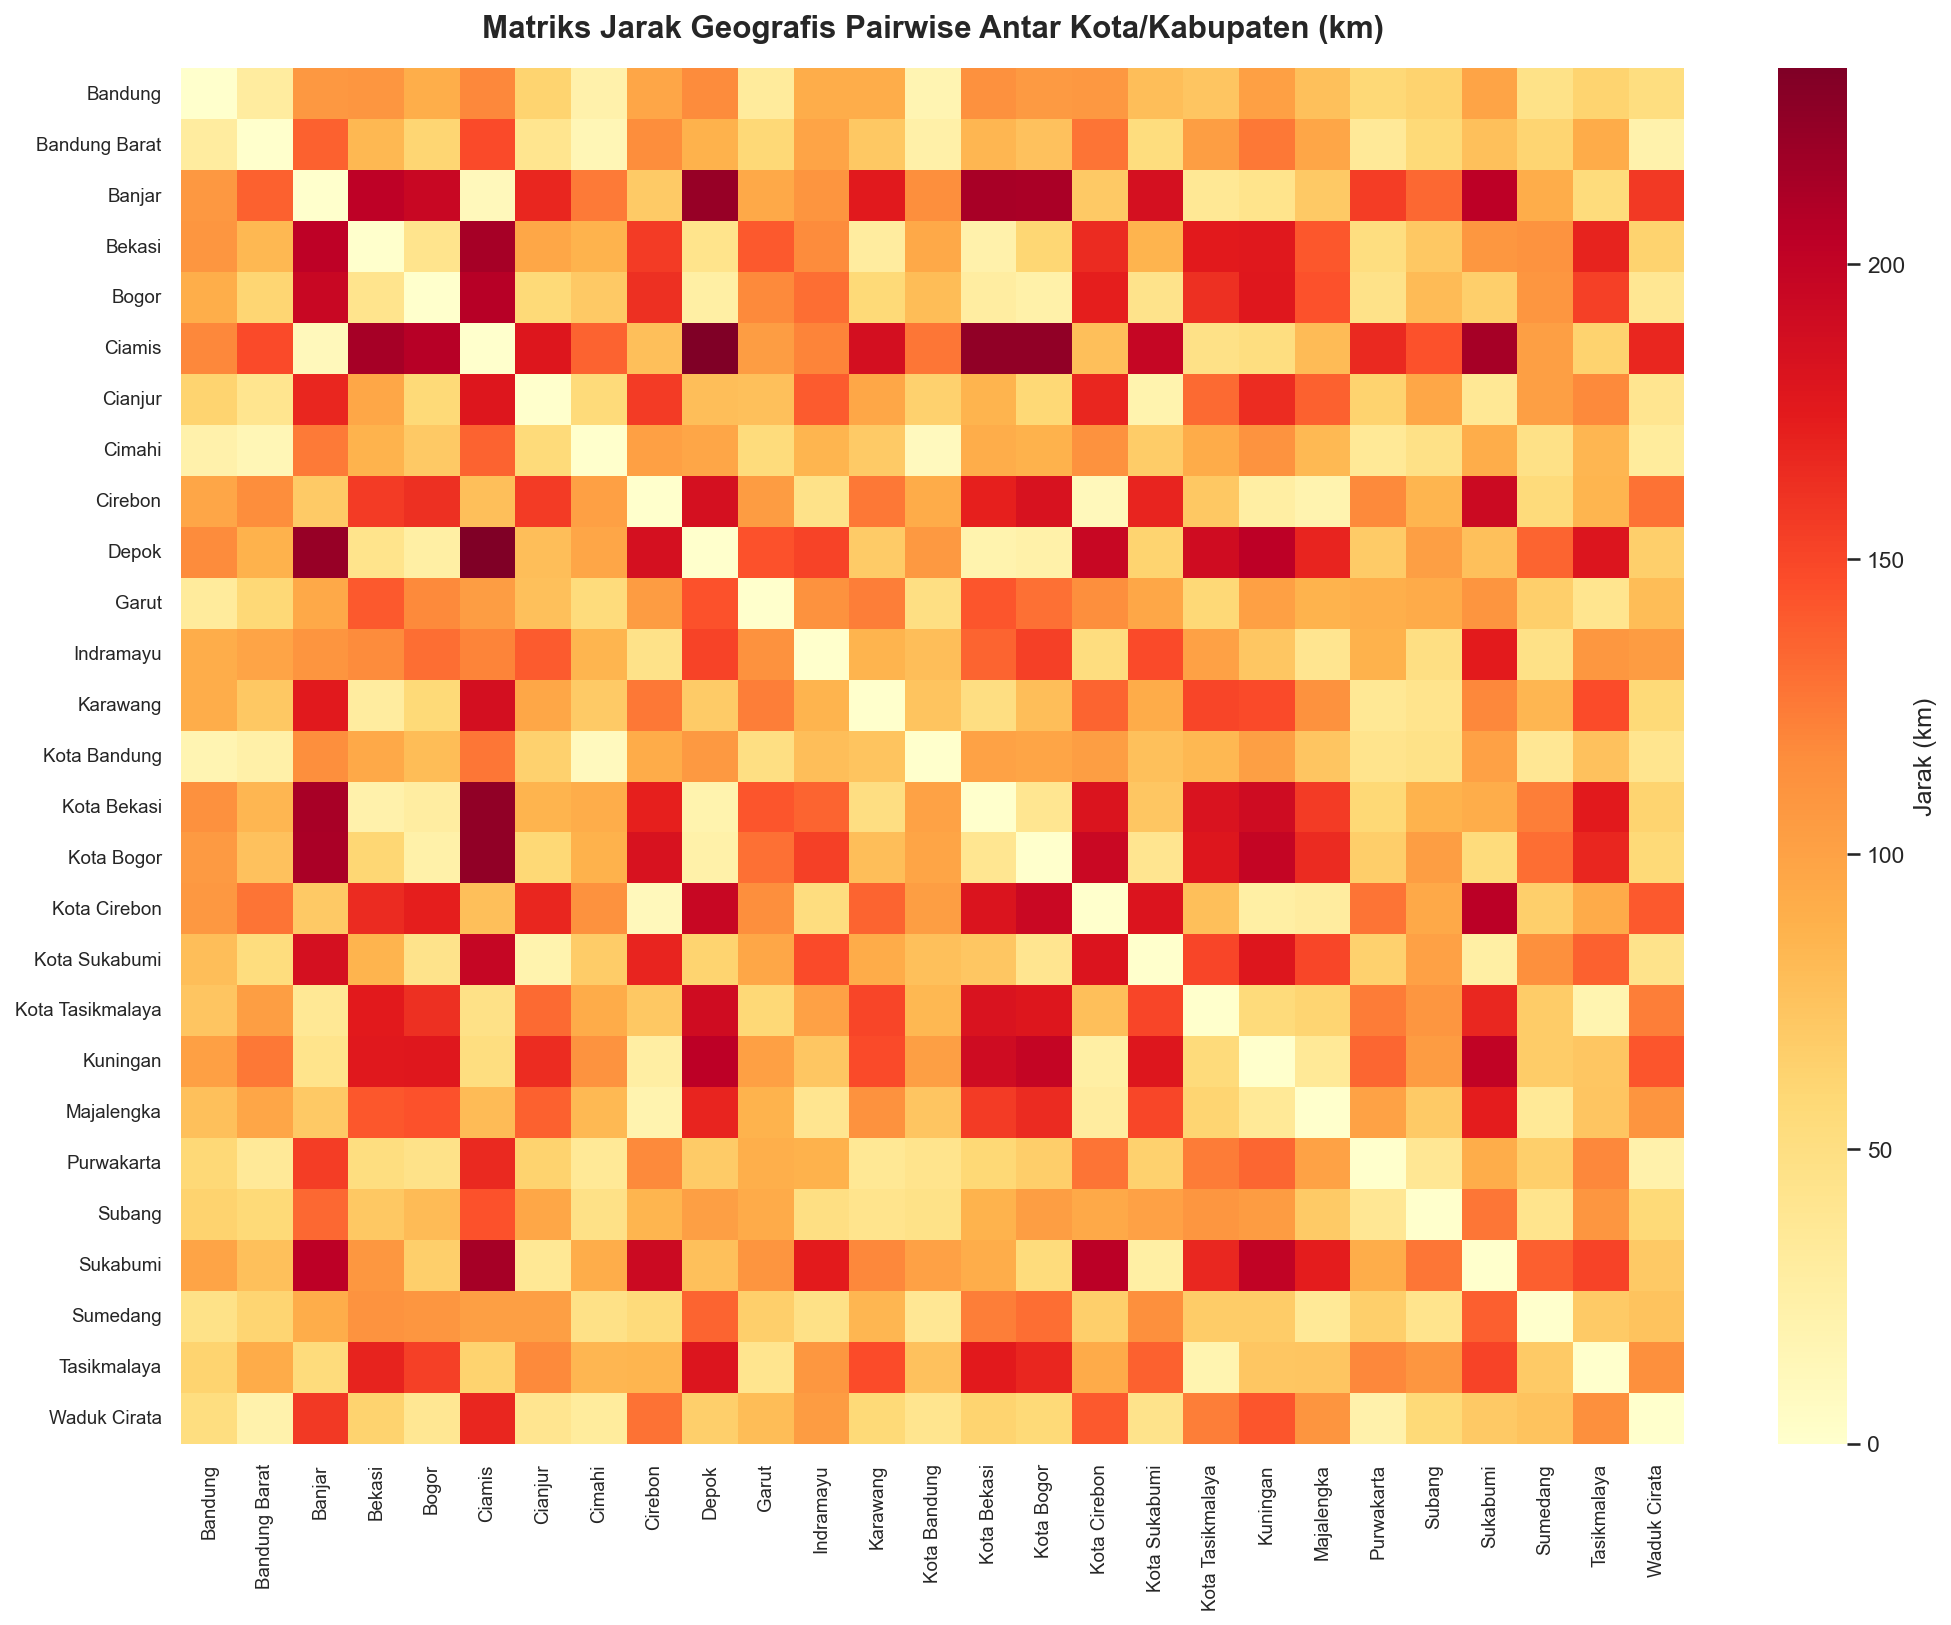
\includegraphics[width=\linewidth,height=0.65\textheight,keepaspectratio]{04_matriks_jarak_geografis.png}
    {\scriptsize\color{Slate} Heatmap jarak antar kota menunjukkan kluster wilayah}
  \end{columns}
\end{frame}

% ─────────────────────────────────────────────
%  SLIDE 5 · Baseline Greedy
% ─────────────────────────────────────────────
\begin{frame}{Baseline: \textit{Greedy Nearest Neighbor}}
  \begin{columns}[T]
    \column{0.5\textwidth}
    \textbf{Pendekatan Pembanding (Heuristik Lokal)}
    \begin{enumerate}
      \item Memulai dari kota awal.
      \item Selalu memilih kota terdekat yang belum dikunjungi.
      \item Mengulangi hingga seluruh kota dikunjungi, lalu kembali ke titik awal.
    \end{enumerate}
    
    \vspace{0.2cm}
    \textbf{Kelebihan:} Sederhana dan cepat (Kompleksitas $\mathcal{O}(n^2)$).
    
    \vspace{0.2cm}
    \textbf{Kekurangan:} Bersifat lokal. Rentan terhadap \textit{local optimum} karena tidak mempertimbangkan konsekuensi jangka panjang (melahirkan lompatan jauh di akhir rute).
    
    \column{0.45\textwidth}
    \vspace{0.5cm}
    \begin{beamercolorbox}[wd=\linewidth,sep=12pt,rounded=true]{block body}
      \centering
      {\large\bfseries Hasil Baseline}\\[8pt]
      Total jarak: \textbf{\color{Sky} 891,94 km}\\[4pt]
      Waktu komputasi: \textbf{\color{Sky} $\approx$2 ms}
    \end{beamercolorbox}
  \end{columns}
\end{frame}

% ─────────────────────────────────────────────
%  SLIDE 6 · Mengapa Memetic PSO
% ─────────────────────────────────────────────
\begin{frame}{Mengapa Memetic PSO?}
  \framesubtitle{Pendekatan Metaheuristik Berbasis Kawanan}
  \begin{columns}[T]
    \column{0.55\textwidth}
    \textit{Particle Swarm Optimization} (PSO) meniru perilaku sosial kawanan hewan (mis. burung) dalam mencari solusi.
    
    Tiap partikel belajar dari:
    \begin{itemize}
      \item \textbf{PBest} (Pengalaman/Jarak terbaik individu)
      \item \textbf{GBest} (Pengalaman/Jarak terbaik seluruh kawanan)
    \end{itemize}
    
    \column{0.4\textwidth}
    \begin{block}{Mengapa PSO?}
      \begin{itemize}
        \item Mengeksplorasi banyak kandidat solusi secara bersamaan (global).
        \item Lebih mampu keluar dari jebakan \textit{local optimum} dibanding algoritma \textit{Greedy}.
      \end{itemize}
    \end{block}
  \end{columns}
  
  \vspace{0.5cm}
  \begin{beamercolorbox}[wd=\linewidth,sep=8pt,rounded=true]{block body}
    \centering\small
    \textbf{Strategi Memetic:} Greedy cepat menemukan solusi awal yang logis, sedangkan integrasi PSO \& \textit{Local Search} berupaya mengoptimalkan solusi tersebut secara global.
  \end{beamercolorbox}
\end{frame}

% ─────────────────────────────────────────────
%  SLIDE 7 · Adaptasi PSO
% ─────────────────────────────────────────────
\begin{frame}{Adaptasi PSO untuk TSP}
  \framesubtitle{\textit{Discrete Particle Swarm Optimization}}
  Karena TSP berupa \textbf{permutasi urutan kota} (diskrit), PSO kontinu dimodifikasi menggunakan aljabar \textbf{\textit{Swap Operator}}.
  
  \vspace{0.2cm}
  \begin{itemize}
    \item \textbf{Posisi ($X$)} $\rightarrow$ Urutan kota (Contoh: \texttt{[0, 1, 2, 3]})
    \item \textbf{Kecepatan ($V$)} $\rightarrow$ Urutan operasi pertukaran / \textit{swap} (Contoh: \texttt{swap(1, 3)})
  \end{itemize}
  
  \vspace{0.3cm}
  \begin{block}{Persamaan Pembaruan}
    \[
      V_{t+1}=wV_t+c_1r_1(PBest-X)+c_2r_2(GBest-X)
    \]
    \[
      X_{t+1}=X_t+V_{t+1}
    \]
  \end{block}
  \vspace{0.1cm}
  \centering\small\color{Slate} Tiap iterasi, kecepatan partikel ditambahkan ke posisinya sehingga rute makin mendekati PBest dan GBest.
\end{frame}

% ─────────────────────────────────────────────
%  SLIDE 8 · Rancangan Memetic
% ─────────────────────────────────────────────
\begin{frame}{Rancangan Memetic PSO}
  \framesubtitle{5 Strategi Optimasi Hibrida}
  Untuk meningkatkan kualitas solusi dan mencegah konvergensi prematur, PSO dipadukan dengan lima teknik optimasi:
  
  \vspace{0.3cm}
  \begin{tabular}{@{}ll@{}}
    \toprule
    \textbf{Teknik} & \textbf{Tujuan / Mekanisme} \\
    \midrule
    \textbf{Heuristic Seeding} & Memulai Partikel-0 dari rute \textit{Greedy} agar memiliki awalan yang kuat. \\
    \textbf{Velocity Cap}      & Membatasi jumlah maksimal \textit{swap} agar pergerakan partikel stabil. \\
    \textbf{Periodic 2-opt}    & Memperbaiki \textit{crossing edge} pada rute partikel \textit{elite} tiap 5 iterasi. \\
    \textbf{Adaptive Mutation} & Menyeimbangkan fase eksplorasi (awal) dan eksploitasi (akhir). \\
    \textbf{Partial Restart}   & Me-reset sebagian partikel terburuk saat \textit{swarm} stagnan (CoV $<1\%$). \\
    \bottomrule
  \end{tabular}
  
  \vspace{0.4cm}
  \centering\small\color{Slate} Kombinasi eksplorasi, eksploitasi, dan pencarian lokal (\textit{2-opt}) meningkatkan performa PSO secara drastis.
\end{frame}

% ─────────────────────────────────────────────
%  SLIDE 9 · Alur Implementasi
% ─────────────────────────────────────────────
\begin{frame}{Alur Implementasi Sistem}
  \begin{center}
    \begin{tikzpicture}[
      >=Latex,
      box/.style={draw=Sky, rounded corners=6pt, fill=Mist,
                  minimum width=2.4cm, minimum height=0.72cm,
                  align=center, font=\small, text=Ink}
    ]
      \node[box] (d) {Dataset 27 Kota};
      \node[box, right=0.5cm of d] (h) {Perhitungan\\Haversine};
      \node[box, right=0.5cm of h] (g) {Greedy\\Baseline};
      \node[box, right=0.5cm of g] (t) {Auto-Tuning\\PSO};
      
      \node[box, below=1cm of t] (p) {Memetic PSO};
      \node[box, left=0.5cm of p] (e) {Evaluasi \&\\Analisis};
      \node[box, left=0.5cm of e] (v) {Visualisasi\\Interaktif};

      \draw[->, thick, Sky] (d) -- (h);
      \draw[->, thick, Sky] (h) -- (g);
      \draw[->, thick, Sky] (g) -- (t);
      \draw[->, thick, Sky] (t) -- (p);
      \draw[->, thick, Sky] (p) -- (e);
      \draw[->, thick, Sky] (e) -- (v);
    \end{tikzpicture}
  \end{center}
  
  \vspace{0.5cm}
  \textbf{Komponen Implementasi:}
  \begin{itemize}
    \item \textbf{Core Algorithm} (\texttt{pso\_engine.py}) $\rightarrow$ Berbasis OOP dengan \textit{type hints}.
    \item \textbf{Notebook Eksperimen} $\rightarrow$ Analisis spasial \& konvergensi (\textit{Matplotlib/Seaborn}).
    \item \textbf{Dashboard Interaktif} (\texttt{app.py}) $\rightarrow$ Aplikasi \textit{Streamlit} dengan \textit{Plotly Mapbox}.
  \end{itemize}
\end{frame}

% ─────────────────────────────────────────────
%  SLIDE 10 · Setup Eksperimen
% ─────────────────────────────────────────────
\begin{frame}{Setup Eksperimen \& Auto-Tuning}
  Empat \textit{preset} dievaluasi secara otomatis:
  \textit{Balanced}, \textit{Exploration-Heavy}, \textit{Exploitation-Heavy}, dan \textit{Lightweight}.
  
  \vspace{0.3cm}
  \begin{columns}[T]
    \column{0.45\textwidth}
    \begin{block}{Preset Terbaik: Exploitation Heavy}
      Parameter Utama:
      \begin{itemize}
        \item $w$ (Inersia) = 0,4
        \item $c_1$ (Kognitif) = 1,0
        \item $c_2$ (Sosial) = 2,0
        \item Jumlah partikel = 15
        \item Laju mutasi awal = 0,05
        \item \textit{Early stopping} = Aktif
        \item \textit{Seed} reprodusibilitas = 42
      \end{itemize}
    \end{block}
    
    \column{0.5\textwidth}
    \vspace{0.5cm}
    \textbf{Alasan Pemilihan:}
    \begin{itemize}
      \item Menghasilkan rata-rata jarak terpendek selama proses \textit{auto-tuning}.
      \item Karena partikel-0 disemai oleh rute \textit{Greedy}, kawanan tidak butuh eksplorasi liar, melainkan eksploitasi agresif (tarikan sosial / $c_2$ tinggi) menuju area solusi optimal tersebut.
    \end{itemize}
  \end{columns}
\end{frame}

% ─────────────────────────────────────────────
%  SLIDE 11 · Hasil Eksperimen: Peta Rute
% ─────────────────────────────────────────────
\begin{frame}{Hasil Eksperimen: Perbandingan Rute}
  \begin{columns}[T]
    \column{0.7\textwidth}
    \centering
    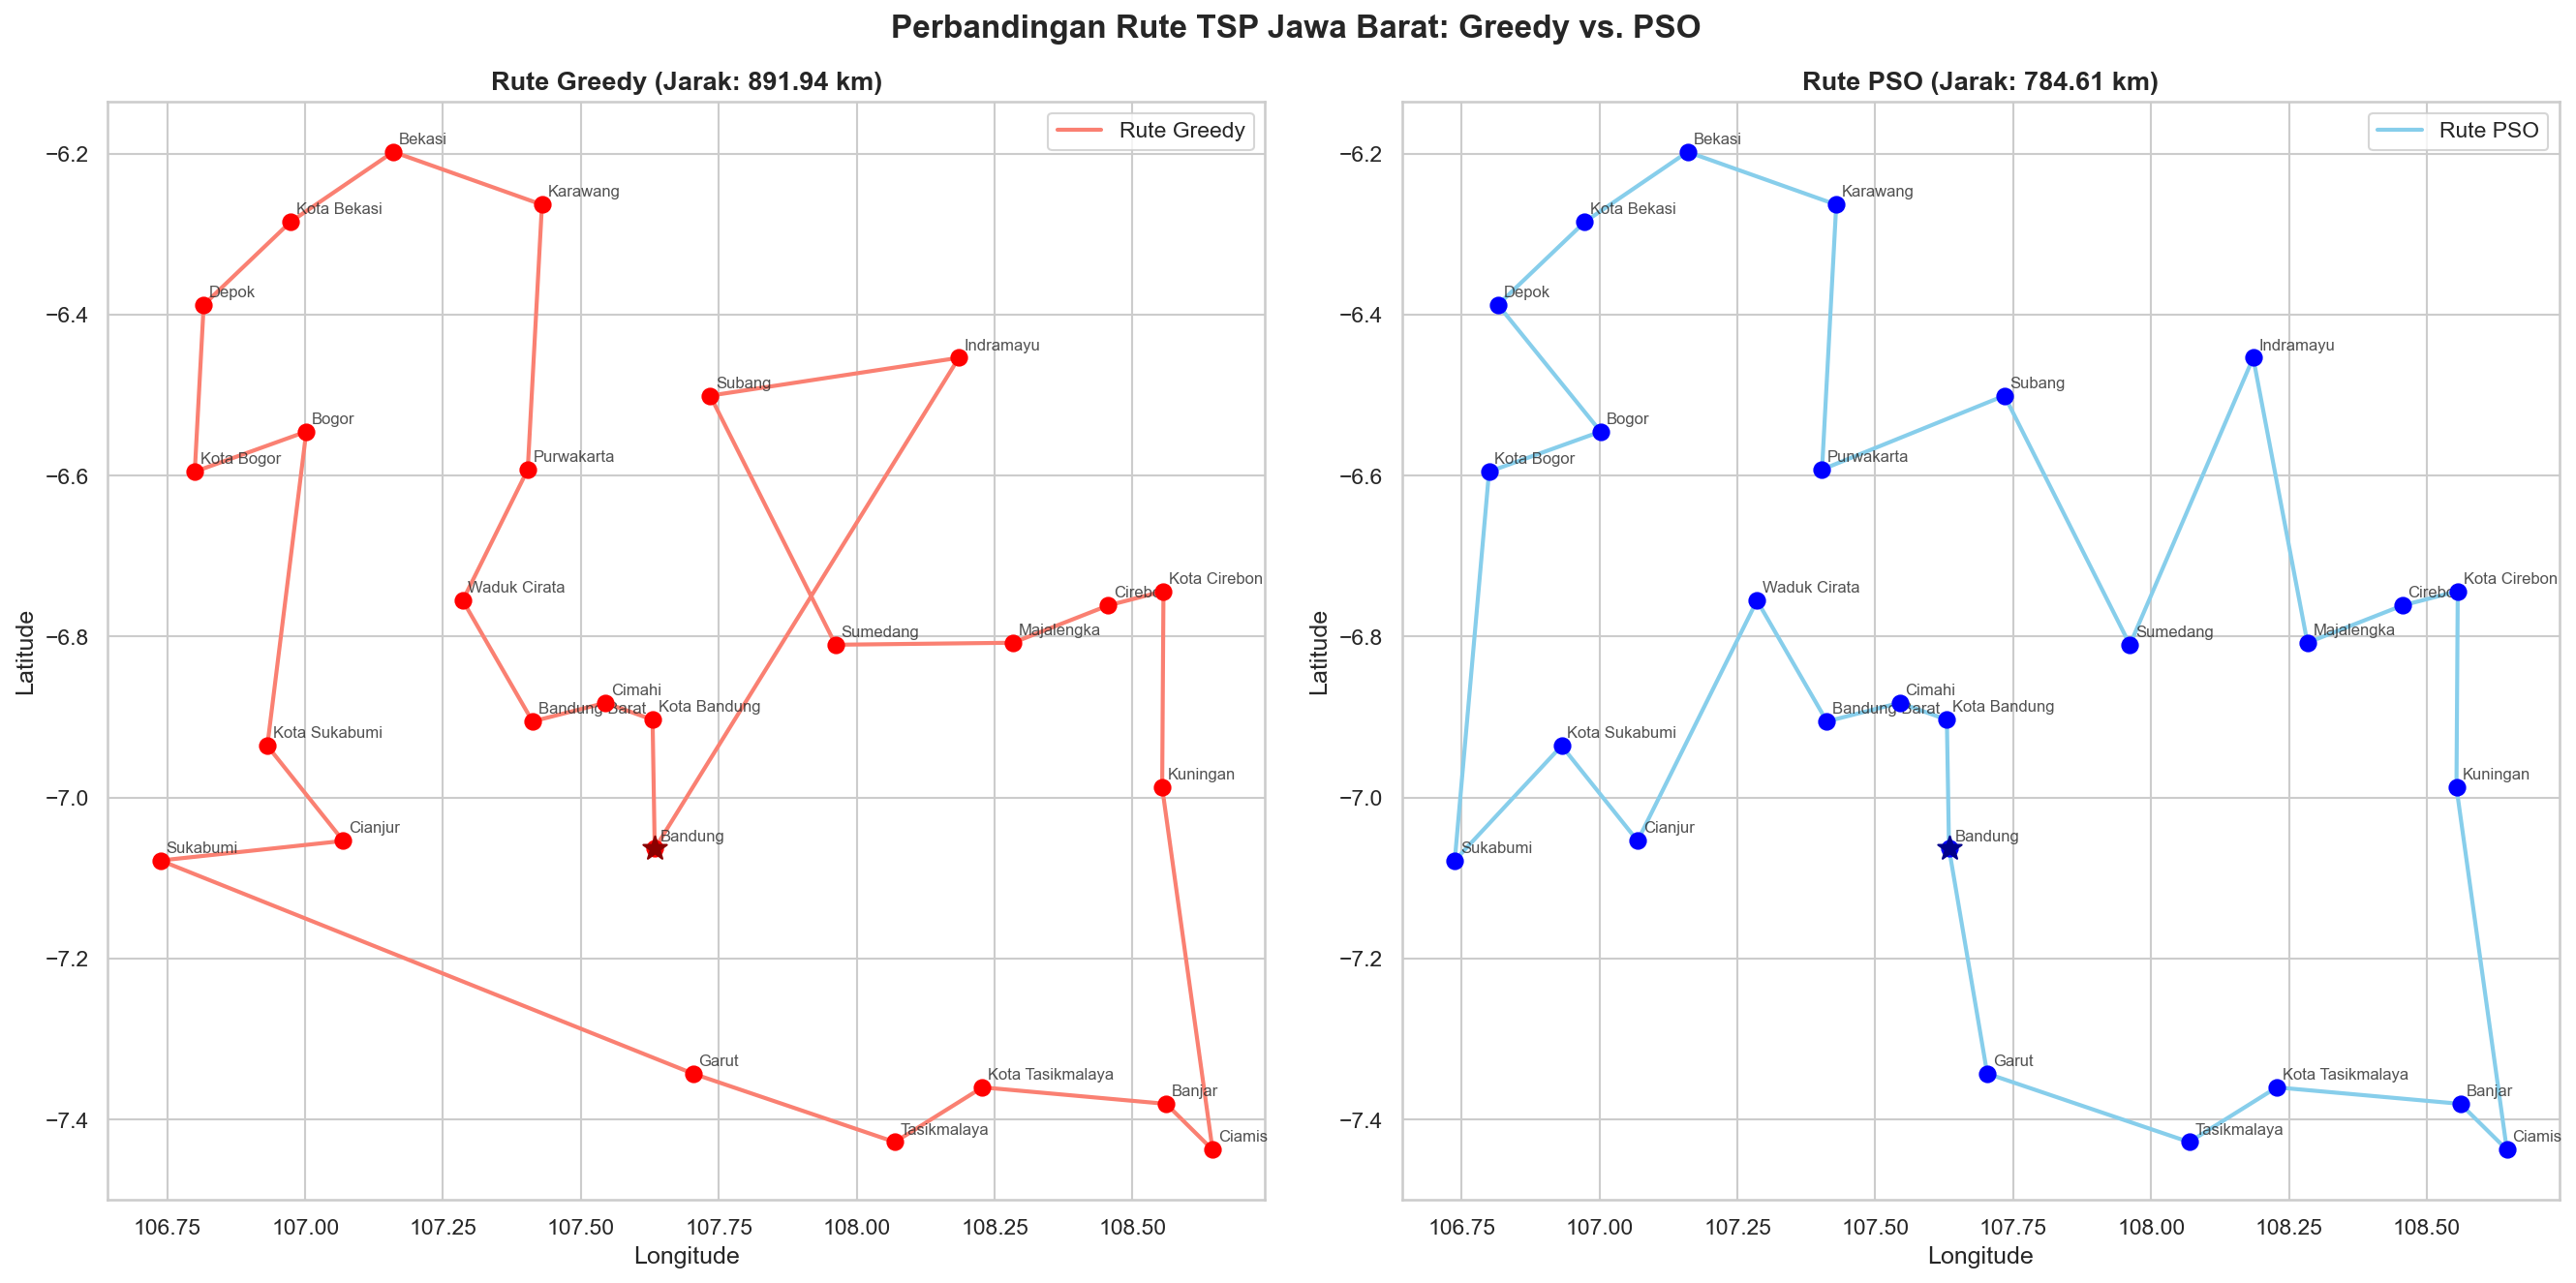
\includegraphics[width=\linewidth,height=0.7\textheight,keepaspectratio]{02_perbandingan_rute_greedy_vs_pso.png}
    
    \column{0.28\textwidth}
    \vspace{0.5cm}
    \begin{block}{Jarak Rute}
      \textbf{Greedy NN:}\\ 891,94 km\\[0.2cm]
      \textbf{Memetic PSO:}\\ \textbf{788,08 km}
    \end{block}
    
    \begin{block}{Peningkatan}
      Penghematan:\\ \textbf{103,86 km}\\[0.2cm]
      Efisiensi:\\ \textbf{11,64\%}
    \end{block}
  \end{columns}
  
  \vspace{0.1cm}
  \centering\small\color{Slate}
  \textbf{Interpretasi Visual:} \textit{Crossing edge} berkurang drastis, PSO mengikuti kedekatan geografis lebih logis.
\end{frame}

% ─────────────────────────────────────────────
%  SLIDE 12 · Hasil Eksperimen: Konvergensi
% ─────────────────────────────────────────────
\begin{frame}{Hasil Eksperimen: Kurva Konvergensi}
  \begin{columns}[T]
    \column{0.65\textwidth}
    \centering
    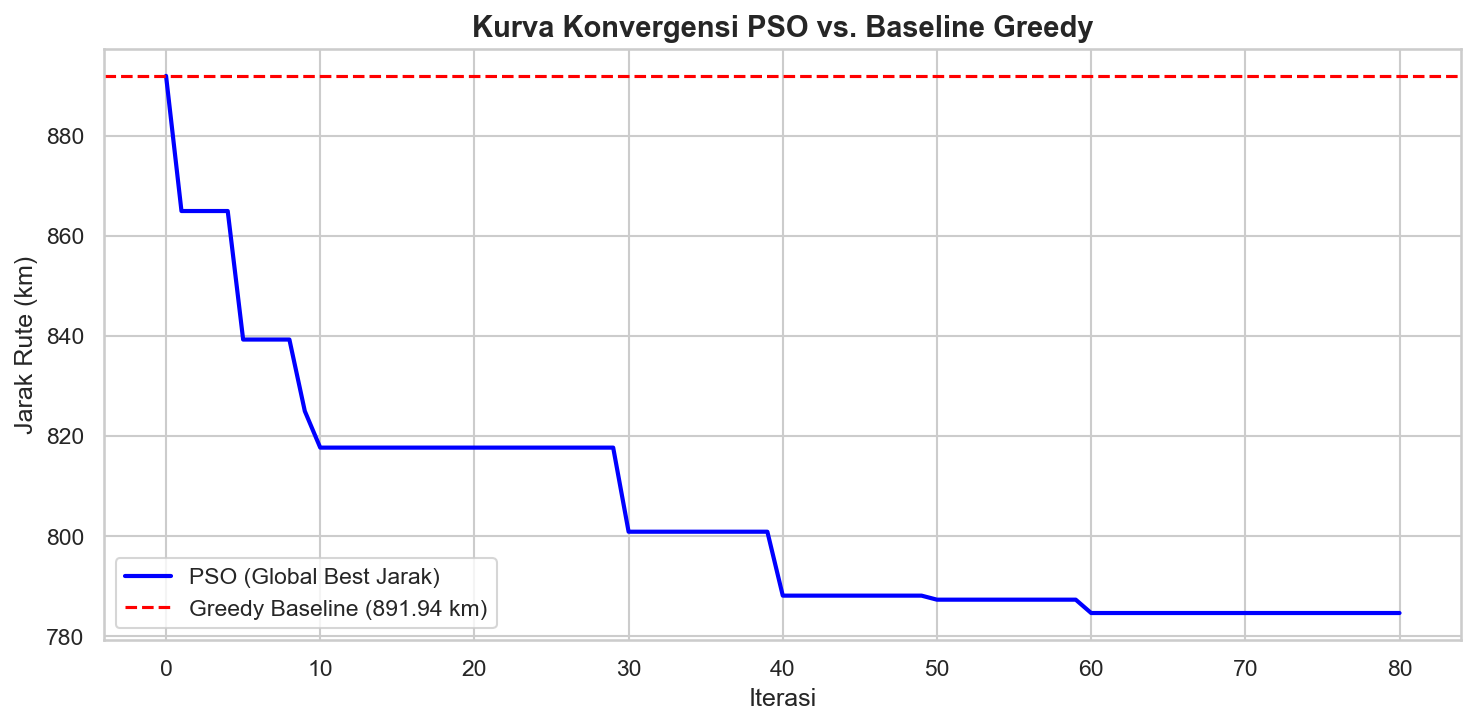
\includegraphics[width=\linewidth,height=0.75\textheight,keepaspectratio]{01_kurva_konvergensi_pso_vs_greedy.png}
    
    \column{0.32\textwidth}
    \vspace{1cm}
    \textbf{Analisis Kurva:}
    \begin{itemize}
      \item Titik awal PSO (biru) bermula dari batas jarak \textit{Greedy} berkat teknik \textit{heuristic seeding}.
      \item Bantuan operasi \textit{2-opt} periodik memotong jarak secara masif.
      \item Sistem konvergen penuh dan berhenti di iterasi ke-60 akibat \textit{early stopping}.
    \end{itemize}
  \end{columns}
\end{frame}

% ─────────────────────────────────────────────
%  SLIDE 13 · Analisis Kinerja
% ─────────────────────────────────────────────
\begin{frame}{Validasi Akademik: Analisis Kinerja Eksekusi}
  \begin{columns}[T]
    \column{0.65\textwidth}
    \centering
    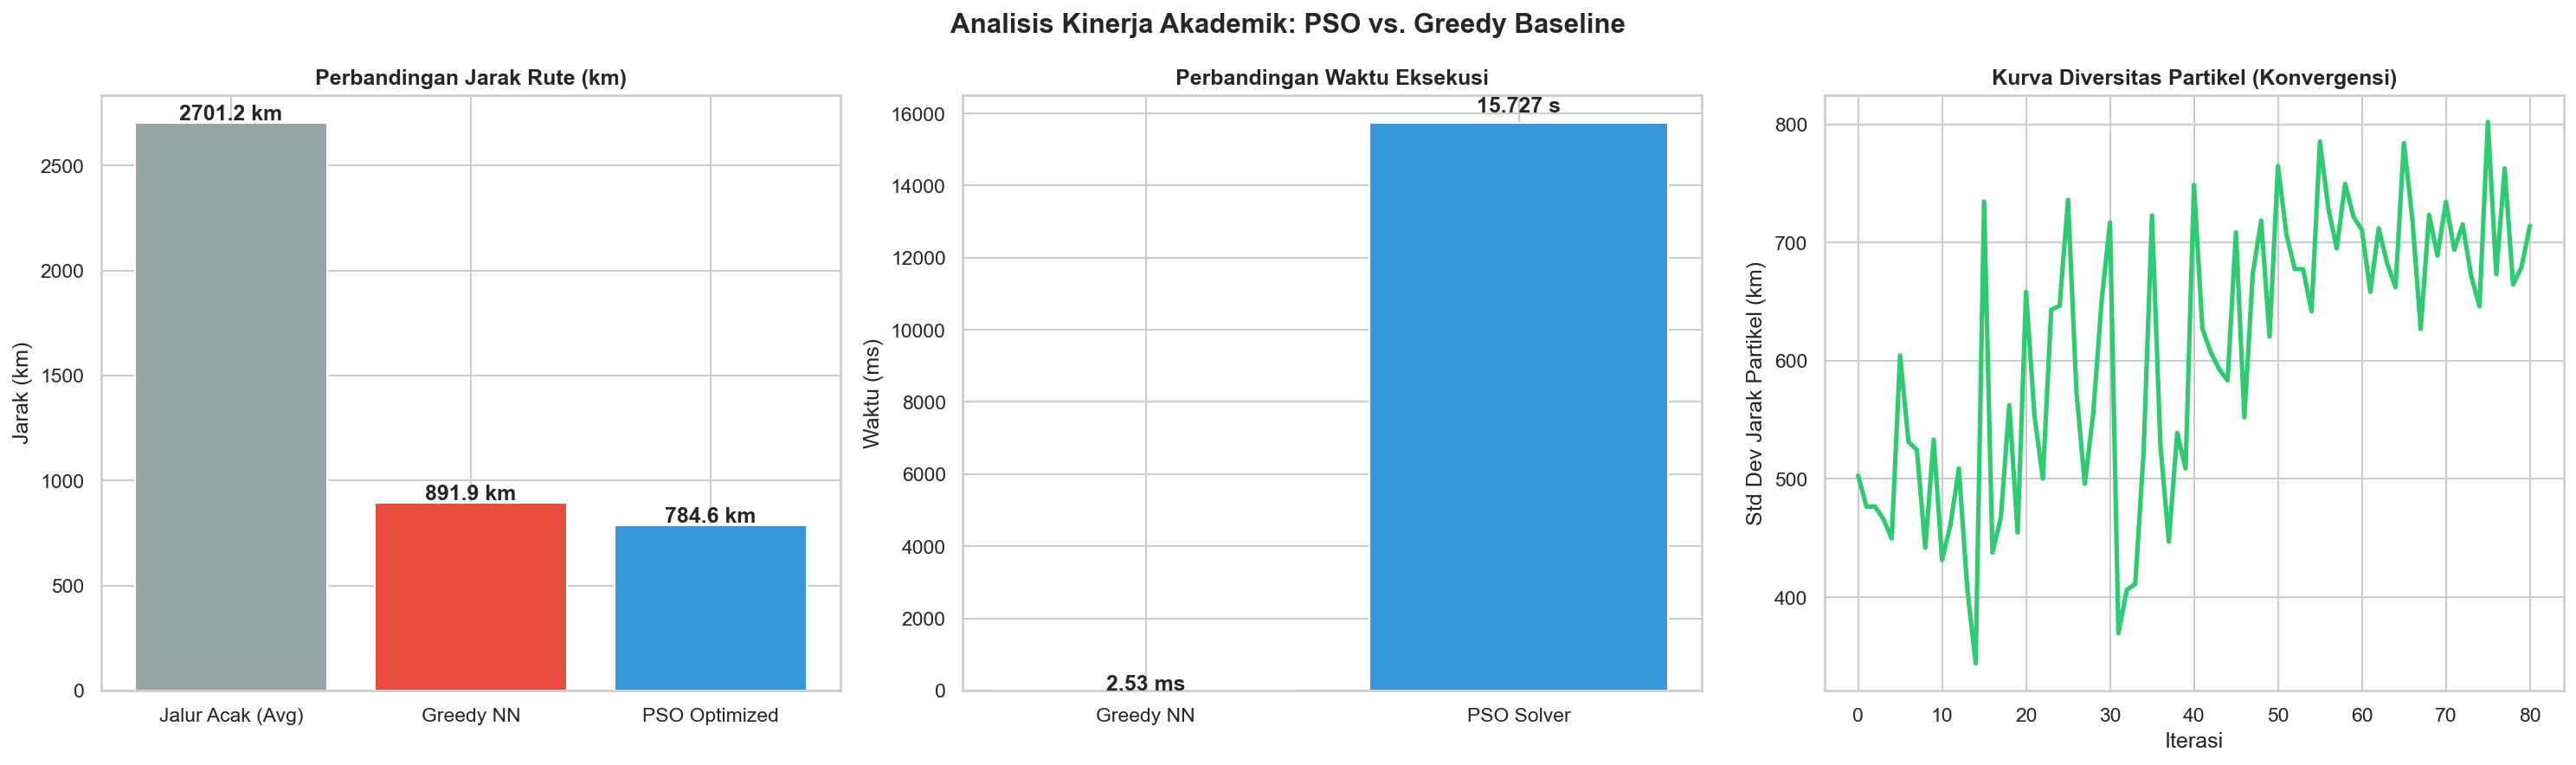
\includegraphics[width=\linewidth,height=0.75\textheight,keepaspectratio]{03_analisis_kinerja_pso_vs_greedy.png}
    
    \column{0.32\textwidth}
    \vspace{0.5cm}
    \textbf{Trade-off Waktu (Tengah):}
    \begin{itemize}
      \item Waktu PSO sedikit lebih lambat dari Greedy ($\approx 10$ s), namun rasional untuk efisiensi bahan bakar sejauh $>100$ km.
    \end{itemize}
    \vspace{0.3cm}
    \textbf{Diversitas Swarm (Kanan):}
    \begin{itemize}
      \item Variansi antar partikel menurun konsisten ke titik 0, membuktikan kawanan benar-benar \textit{konvergen} (sepakat) pada solusi tersebut.
    \end{itemize}
  \end{columns}
\end{frame}

% ─────────────────────────────────────────────
%  SLIDE 14 · Validasi Spasial
% ─────────────────────────────────────────────
\begin{frame}{Validasi Akademik: Analisis Spasial (\textit{Edge Hop Length})}
  \begin{columns}[T]
    \column{0.65\textwidth}
    \centering
    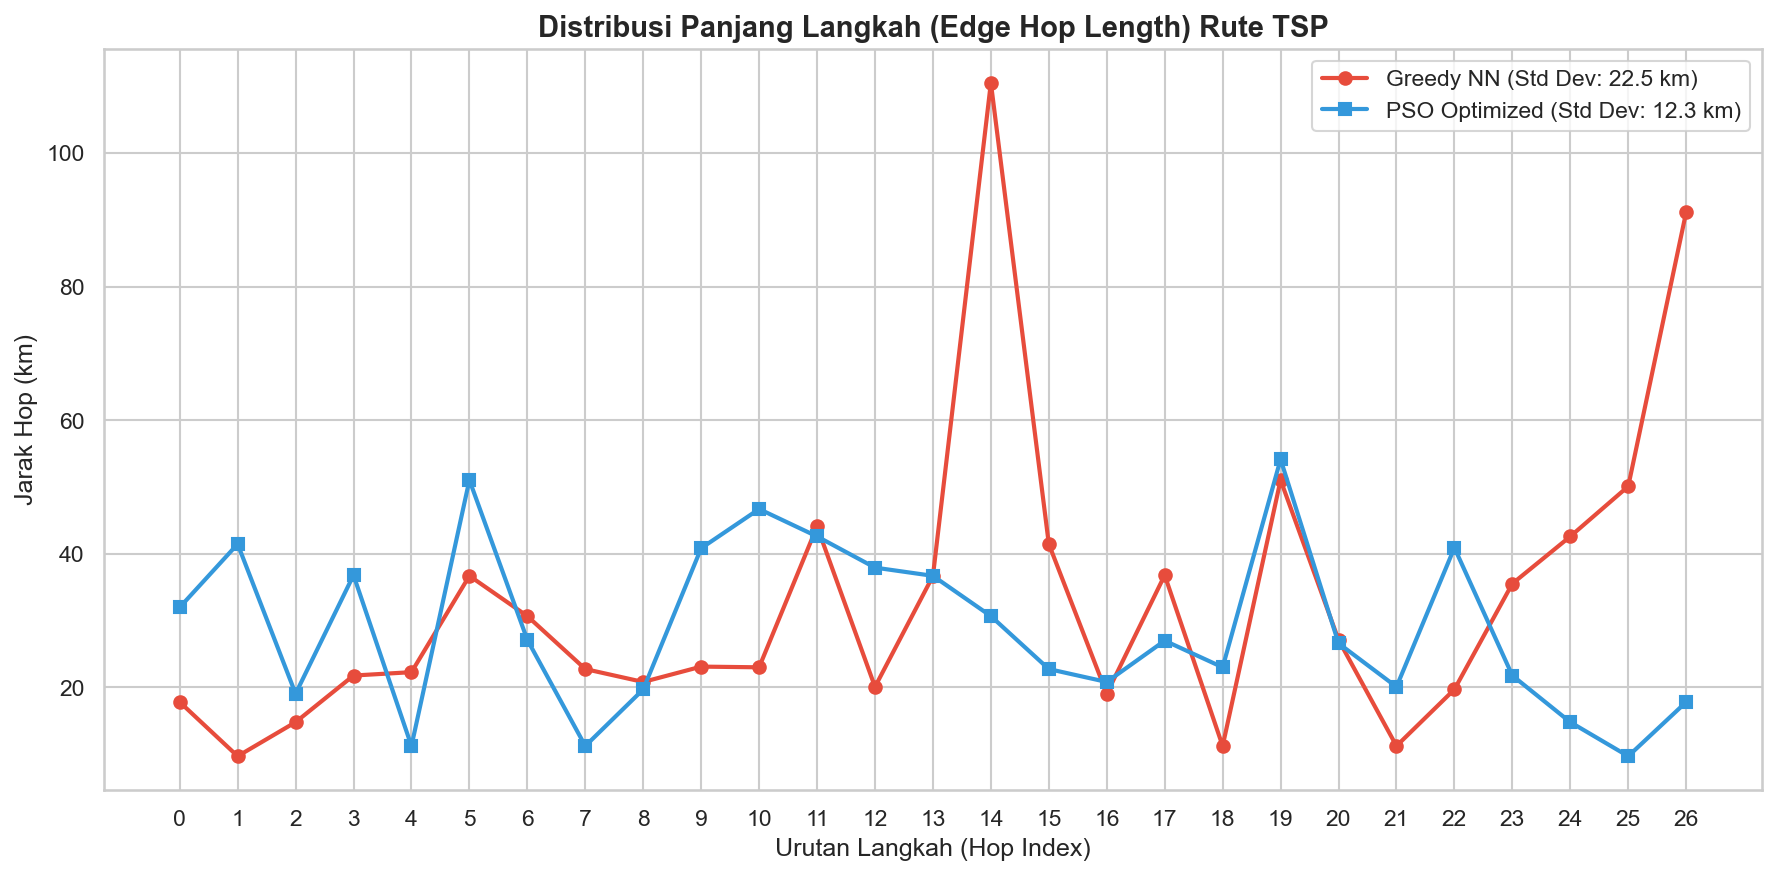
\includegraphics[width=\linewidth,height=0.75\textheight,keepaspectratio]{05_distribusi_panjang_langkah_rute.png}
    
    \column{0.32\textwidth}
    \vspace{0.5cm}
    \textbf{Greedy (Merah):}
    \begin{itemize}
      \item Menghasilkan anomali langkah ekstrem $>100$ km akibat kota yang tertinggal dikunjungi di akhir rute.
    \end{itemize}
    \vspace{0.3cm}
    \textbf{PSO (Biru):}
    \begin{itemize}
      \item Distribusi jarak antar-kota sangat padat di titik pendek (Standar Deviasi mengecil).
      \item Membuktikan PSO berhasil mengeksploitasi intra-kluster wilayah dengan cermat.
    \end{itemize}
  \end{columns}
\end{frame}

% ─────────────────────────────────────────────
%  SLIDE 15 · Kesimpulan & Pengembangan
% ─────────────────────────────────────────────
\begin{frame}{Kesimpulan, Keterbatasan, dan Pengembangan}
  \begin{block}{Kesimpulan}
    \begin{itemize}
      \item Memetic PSO sukses besar memecahkan jebakan \textit{local optimum} algoritma \textit{Greedy}.
      \item Total jarak berhasil direduksi dari \textbf{891,94 km} menjadi \textbf{788,08 km} (efisiensi \textbf{11,64\%}).
      \item Hibridisasi \textit{Discrete PSO}, \textit{Greedy Seeding}, dan pencarian lokal \textit{2-opt} terbukti luar biasa tangguh untuk optimasi TSP geografis riil.
    \end{itemize}
  \end{block}

  \begin{columns}[T]
    \column{0.5\textwidth}
    \textbf{Keterbatasan:}
    \begin{itemize}
      \item Waktu komputasi lebih tinggi.
      \item Sangat sensitif terhadap konfigurasi parameter (*tuning*).
      \item Tetap berpotensi sebagai \textit{local optimum} (tidak absolut global).
    \end{itemize}
    
    \column{0.5\textwidth}
    \textbf{Pengembangan Mendatang:}
    \begin{itemize}
      \item Membangun fungsi kebugaran yang berbasis \textbf{waktu tempuh jalan raya riil} (menggunakan Google Maps/OSRM API), bukan sekadar jarak vertikal udara (*Haversine*).
    \end{itemize}
  \end{columns}
\end{frame}

% ─────────────────────────────────────────────
%  SLIDE 16 · Penutup
% ─────────────────────────────────────────────
\begin{frame}[plain]
  \begin{tikzpicture}[remember picture,overlay]
    \fill[Ink] (current page.south west) rectangle (current page.north east);
    \fill[Sky]           ([xshift=-1.6cm,yshift=1.0cm]current page.south east) circle (1.35cm);
    \fill[white,opacity=0.08] ([xshift=1.8cm,yshift=-1.0cm]current page.north west) circle (2.0cm);
    \fill[Sky,opacity=0.25]   ([xshift=5.5cm,yshift=-1.8cm]current page.north west) circle (0.9cm);
  \end{tikzpicture}

  \vspace{1.8cm}
  \centering
  {\color{white}\Huge\bfseries Terima Kasih}

  \vspace{0.5cm}
  {\color{white!80}\large Sesi Diskusi dan Tanya Jawab}

  \vspace{0.8cm}
  {\color{white!55}\footnotesize
    Naufal Akmal Rizqulloh \quad Adhiya Radhin Fasya \quad Faiz Naufal Huda\\[4pt]
    Insan Anshary Rasul \quad Daffa Naufal Mumtaz
  }
\end{frame}

\end{document}
